\section{Análisis comparativo}

En las secciones anteriores pudimos ver el desempeño de cada filtro por separado, veamos ahora la comparativa utilizando las medidas PESQ y STOI. En la figura \ref{fig:ch8_pesq_comparison} podemos ver la variación media en la PESQ, tanto para el filtro adaptativo como para el filtro neuronal para los distintos niveles de ruidos utilizados.

\begin{figure}
	\centering
	\centerline{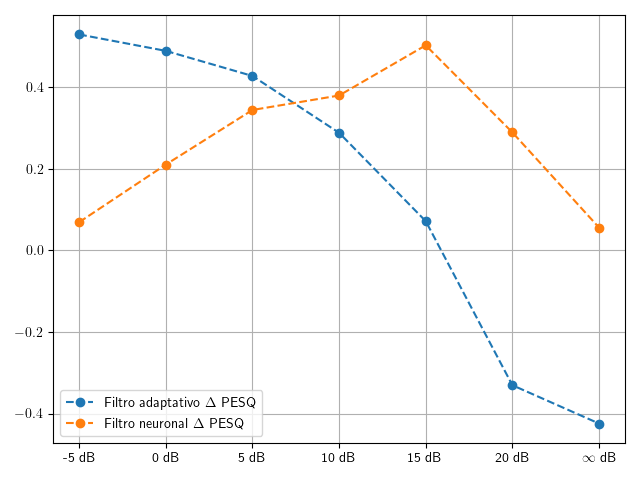
\includegraphics[scale=0.75]{images/ch8/comparison_pesq.png}}
	\caption{Comparación PESQ}
	\label{fig:ch8_pesq_comparison}
\end{figure}

Para el caso del filtro adaptativo vemos que el mejor desempeño se obtuvo para un SNR de \SI{-5}{dB} y para SNRs mayores, la variación media disminuyó. La disminución en el desempeño a medida que aumenta la SNR se debe al error en estado estacionario del filtro adaptativo como vimos en la figura \ref{fig:ch6_mse_and_noise_level}.

Por otro lado, el filtro neuronal logra el mejor desempeño para los \SI{15}{dB} y con un valor similar al del caso del filtro adaptativo. A diferencia del filtro adaptativo, tanto para SNRs altos como para bajos el desempeño disminuyó respecto del obtenido para \SI{15}{dB}. La disminución en el desempeño, en bajos niveles de SNR, se debe a los errores de estimación en el espectro y en altos niveles de SNR, al error de generalización de la red, como vimos en la figura \ref{fig:ch7_mse_and_noise_level}.	

En la figura \ref{fig:ch8_stoi_comparison} podemos ver la variación media en la STOI, tanto para el filtro adaptativo como para el filtro neuronal para los distintos niveles de ruidos utilizados.

\begin{figure}
	\centering
	\centerline{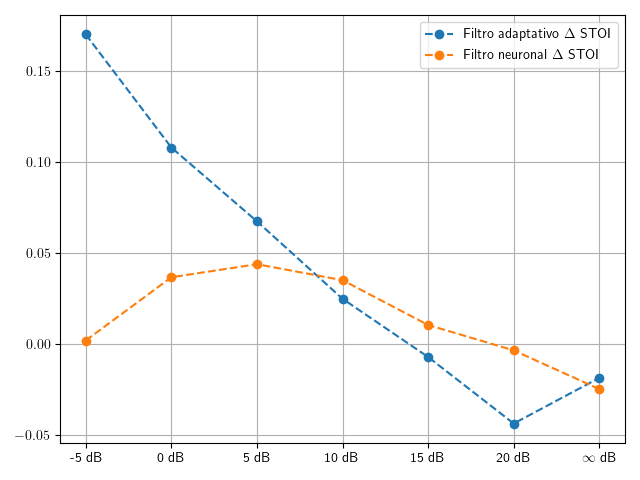
\includegraphics[scale=0.75]{images/ch8/comparison_stoi.png}}
	\caption{Comparación STOI}
	\label{fig:ch8_stoi_comparison}
\end{figure}

Para el caso de la STOI se obtuvieron características similares que para la PESQ, es decir, el filtro adaptativo tuvo un mejor desempeño a bajos niveles de SNR y el filtro neuronal se desempeñó mejor que el adaptativo a niveles altos de SNR. A diferencia de la PESQ, en este caso el desempeño del filtro adaptativo a bajos niveles de SNR fue muy superior. La máxima variación en la STOI para el filtro adaptativo es más de 3 veces la máxima variación en la STOI para el filtro neuronal.